%%%%%%%%%%%%%%%%%%%%%%%%%%%%%%%%%%%%%%%%%%%%%%%%%%%%%%%%%%%%
\section{Kompilierung der Vorlage}%
\label{sec:Kompilierung}
%%%%%%%%%%%%%%%%%%%%%%%%%%%%%%%%%%%%%%%%%%%%%%%%%%%%%%%%%%%%
%
Um diese Vorlage nutzen zu können, benötigt man eine \LaTeX-Distribution (z.B. \printswname{MiKTeX}\footnote{\url{http://www.miktex.org/}} oder \printswname{TeXLive}\footnote{\url{https://tug.org/texlive/acquire.html}}).
Sofern man nicht die riesengroße Komplettinstallation wählt, wird beim ersten Kompilieren eine Internet"=Verbindung benötigt, um Zusatz"=\glspl{gls:pkg} dynamisch nachladen zu können.
Zur Erstellung des Glossars und des Abkürzungsverzeichnisses wird zusätzlich Perl benötigt.
Unter Windows müsste hierzu zusätzlich beispielsweise \printswname{ActivePerl}\footnote{\url{https://www.activestate.com/products/activeperl/}}
oder \printswname{StrawberryPerl}\footnote{\url{http://strawberryperl.com/}} installiert werden.
Bei den Linux-Distributionen ist Perl automatisch mit dabei.

Zur bequemen Bearbeitung der \LaTeX"=Quellcode"=Dateien empfiehlt sich Verwendung einer guten \LaTeX"=Entwicklungsumgebung in Kombination mit einem geeigneten, sprich SyncTeX"=fähigen, PDF"=Betrachter.
Manche Entwicklungsumgebungen bieten eine integrierte PDF"=Vorschau, welche Vor- und Nachteile haben kann.
Ein wichtiges Kriterium bei der Wahl der Entwicklungsumgebung ist die Möglichkeit, zwischen den einzelnen Stellen im Quellcode und im PDF hin- und her springen zu können.
Unter Windows war lange Zeit \textbf{TeXnicCenter}\footnote{\url{http://www.texniccenter.org/}} in Kombination mit \printswname{SumatraPDF}\footnote{\url{https://www.sumatrapdfreader.org}} eine gute Wahl gewesen.
Mittlerweile tendieren die meisten dazu, \printswname{TeXstudio}\footnote{\url{https://www.texstudio.org/}} zu verwenden.
Diese bietet eine eingebaute PDF"=Vorschau und viele nützliche Features und ist sowohl unter Windows als auch unter Linux verfügbar.

%%%%%%%%%%%%%%%%%%%%%%%%%%%%%%%%%%%%%%%%%%%%%%%%%%%%%%%%%%%%
\subsection{MiKTeX-Einstellungen}
\label{sec:MiKTeX}
%%%%%%%%%%%%%%%%%%%%%%%%%%%%%%%%%%%%%%%%%%%%%%%%%%%%%%%%%%%%
Sofern MiKTeX als \LaTeX"=Distribution verwendet wird, sollte man darauf achten, dass bei Bedarf Zusatzpakete vom Internet dynamisch nachgeladen werden können.
Sofern diese Option nicht bei der Installation gesetzt worden ist, kann sie nachträglich in der MiKTeX-Console aktiviert werden.
Zu finden ist diese im Startmenü unter \enquote{MiKTeX}, \enquote{MiKTeX Console (Admin)}.
Unter \enquote{Settings} findet sich ein Reiter \enquote{General}, wo im Bereich \enquote{Package installation} entweder die Option \enquote{Always install missing packages on the fly} oder \enquote{Ask me} ausgewählt werden soll.
Sofern sich der Rechner im Netzwerk des Fraunhofer IOSB befindet, muss zusätzlich noch die Proxy-Option korrekt gesetzt werden.
Hierfür muss man im Bereich \enquote{Package installation} der MiKTeX Console auf \enquote{Change} gehen und bei \enquote{Connection Settings} die Verwendung des Proxy-Servers \printkeyword{proxy-ka.iosb.fraunhofer.de} mit Port \printkeyword{80} aktivieren (s. \cref{fig:MiKTeX-Proxy}).
Wird dies nicht gemacht, können benötigte Pakete nicht nachgeladen werden.

\begin{figure}[htb]%
\centering%
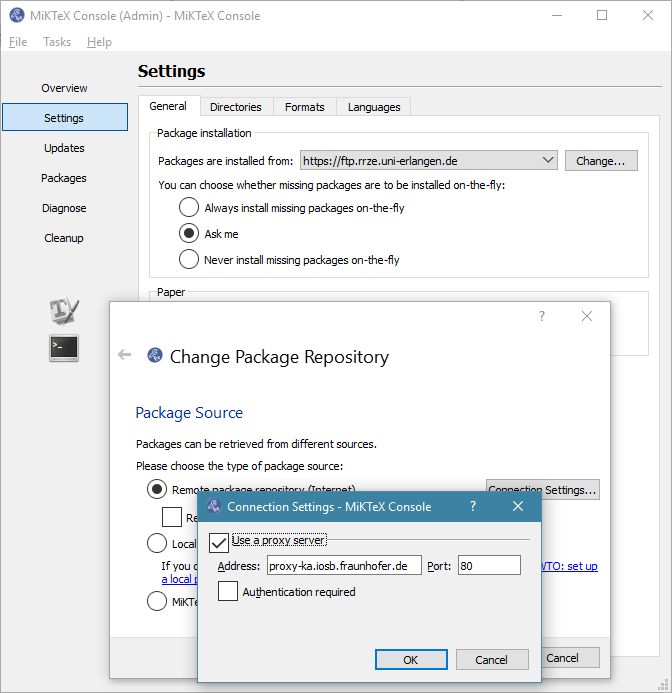
\includegraphics[width=\linewidth]{images/examples/MiKTeX-Proxy.png}%
\caption{MiKTeX-Einstellungen zum Nachladen der Zusatzpakete}%
\label{fig:MiKTeX-Proxy}%
\end{figure}

Nach der MiKTeX-Installation sollte man im Startmenü gleich die MiKTeX-Console aufrufen, den Proxy eintragen und das Update durchführen um die aktuellste Version der vorinstallierten Pakete zu erhalten.
So vermeidet man beim automatischen Nachladen weiterer \glspl{gls:pkg} aus dem \acrshort{ac:CTAN}-Repository etwaige Inkompatibilitäten aufgrund veralteter Stammpakete.


%%%%%%%%%%%%%%%%%%%%%%%%%%%%%%%%%%%%%%%%%%%%%%%%%%%%%%%%%%%%
\subsection{TeXLive-Einstellungen}
\label{sec:TeXLive}
%%%%%%%%%%%%%%%%%%%%%%%%%%%%%%%%%%%%%%%%%%%%%%%%%%%%%%%%%%%%
Bei Verwendung von TeXLive unter Linux muss darauf geachtet werden, dass alle notwendigen Linux-\glspl{gls:pkg} installiert sind.
Unter Ubuntu 17.04 sollte es funktionieren, wenn folgende Linux-\glspl{gls:pkg} installiert wurden:
\begin{itemize*}
	\item \printkeyword{texlive}
	\item \printkeyword{texlive-lang-german}
	\item \printkeyword{texlive-fonts-extra}
	\item \printkeyword{texlive-bibtex-extra}
	\item \printkeyword{fonts-linuxlibertine}
	\item \printkeyword{biber}
	\item \printkeyword{xindy}
	\item \printkeyword{texmaker}
\end{itemize*}
Texmaker ist eine IDE für \LaTeX, die aber vermutlich über Dependencies schon einige Pakete mitbringt.


%%%%%%%%%%%%%%%%%%%%%%%%%%%%%%%%%%%%%%%%%%%%%%%%%%%%%%%%%%%%
\subsection{Kompilieraufrufe}
\label{sec:Aufruf}
%%%%%%%%%%%%%%%%%%%%%%%%%%%%%%%%%%%%%%%%%%%%%%%%%%%%%%%%%%%%
Zur erfolgreichen Kompilierung des Dokumentes müssen mehrere
Kommandozeilenprogramme aufgerufen werden.
Bei Verwendung einer integrierten Entwicklungsumgebung (IDE),
wird diese so konfiguriert, dass die Aufrufe aus der IDE heraus erfolgen und
die etwaigen Warnungen, Erfolgs- und Fehlermeldungen in der IDE sichtbar werden.
Die entsprechenden Einstellungen für TeXnicCenter und TeXstudio finden sich
in den nachfolgenden Kapiteln.

Die einzelnen Aufrufe sind:
\begin{itemize*}
\item \index{xelatex}\printkeyword{xelatex} zur eigentlichen Kompilierung von \LaTeX-Quelltext,
\item \index{biber}\printkeyword{biber} zur Kompilierung von Bibliografien,
\item \index{makeglossaries}\printkeyword{makeglossaries}, welches intern \index{xindy}\printkeyword{xindy} aufruft,
zur Erstellung einer Zwischenausgabe für das Abkürzungsverzeichnis und das Glossar
\index{makexindex}\printkeyword{makeindex}, welches durch die Verwendung des Pakets \pkg{imakeidx} implizit aufgerufen wird, zur Erstellung des Stichwortverzeichnisses
\end{itemize*}
Bei einem Durchlauf von \printkeyword{xelatex}, \printkeyword{biber}, \printkeyword{makeglossaries} und \printkeyword{makeindex}
werden die einzelnen Inhalte sowie die entsprechenden Querverweise
zuerst jeweils in eine oder mehrere Zwischendateien hinausgeschrieben,
die sodann wieder eingelesen und verarbeitet werden müssen.
Manche Inhalte werden daher erst jeweils beim zweiten Aufruf von \printkeyword{xelatex} generiert.
Für die korrekte Generierung eines Dokumentes mit allen Verzeichnissen
(Inhalts-, Abbildungs-, Tabellen-, Literatur, Abkürzungs-, Begriffs und Stichwortverzeichnis),
PDF"=Lesezeichen und korrekt gesetzten Querverweisen,
muss \printkeyword{xelatex} daher mehrmals aufgerufen werden.

Sollte man ausnahmsweise das Dokument doch noch aus der Kommandozeile oder von einem Script heraus aufrufen wollen,
so ist die Reihenfolge der Aufrufe wie folgt:
\begin{verbatim}
#> xelatex -synctex=1 -interaction=nonstopmode Diss.tex
#> biber Diss
#> makeglossaries Diss
#> xelatex -synctex=1 -interaction=nonstopmode Diss.tex
#> xelatex -synctex=1 -interaction=nonstopmode Diss.tex
#> xelatex -synctex=1 -interaction=nonstopmode Diss.tex
\end{verbatim}

Wenn kein \index{Kompilierfehler}Kompilierfehler aufgetreten ist,
sollte nach dem vierten Durchlauf von \printkeyword{xelatex} die
\index{Warnung!Please re-run latex}Warnung \enquote{Please re-run latex}
verschwunden sein.